\begin{exercise}{\emph{(2.6 nel testo)}}
  Considerate il modello in cui $Y_1,\ldots, Y_n$ sono indipendenti e
  identicamente distribuite come una uniforme $Y \sim U(0, \theta)$,
  dove $\theta$ \`e il valore massimo che pu\`o assumere $Y$.
  Determinate per simulazione la distribuzione campionaria di $T = 2Y$
  considerando $\theta = 100, n = 20$. Mostrate con un istogramma che
  la distribuzione dello stimatore \`e approssimabile da una
  normale. Qual \`e la varianza di $T$? Usate questa varianza per
  sovrapporre all'istogramma la curva normale che lo approssima
  (ricordate di disegnare l'istogramma in R con l'opzione freq =
  FALSE).
\end{exercise}
Questo il codice che implementa l'esercizio:
\lstinputlisting{r-sources/exercises/chapter-two/two-six.R}
Vediamo qualche risultato inserendo in R:
\begin{lstlisting}
  > twosix()
  $estimatorVector
    [1]  95.96794 105.40497 110.64482  89.14495 107.99978 116.03221
    94.73158 ...
  
  $empiricalMean
  [1] 100.2173

  $empiricalVar
  [1] 168.8848

  $empiricalVarComputedByHand
  [1] 168.8848

  $sd
  [1] 12.99557
\end{lstlisting}
L'esecuzione della funzione produce la \autoref{fig:two-six}, dove la
curva in blu rappresenta la densit\`a inferita usando gli algoritmi
disponibili in R dello stimatore $2\bar{Y}$, mentre la curva in rosso
rappresenta il modello esatto usando come parametri i valori stimati
dalla media e dalla varianza campionaria (riportate nel precedente
output come \texttt{empiricalMean} e \texttt{empiricalVar}).
\begin{figure}[htb]
\centering
\includegraphics[height=13cm,width=13cm]{r-sources/exercises/chapter-two/two-six.ps}
\caption{Istogramma esercizio 2.6 del testo}
\label{fig:two-six}
\end{figure}

\begin{exercise}{\emph{(2.7 nel testo)}}
  Una azienda chimica ha prodotto un additivo per la benzina che
  dovrebbe migliorare il consumo oltre le 25 miglia per
  gallone. Viene fatto un esperimento con 30 auto uguali su un
  percorso standard e si ottiene un consumo medio di 26.3 mpg con una
  deviazione standard campionaria di 2.4 mpg. Trovare un intervallo di
  confidenza al $95\%$ per il consumo medio supponendo il modello normale.
\end{exercise}
Questo il codice che implementa l'esercizio:
\lstinputlisting{r-sources/exercises/chapter-two/two-seven.R} Nel
campionamento ripetuto l'intervallo di confidenza riportato sotto
conterr\`a il vero valore del parametro (consumo medio) con una
probabilit\`a di copertura del 95\%.
\begin{lstlisting}
  > twoSeven()
  $tOss
  [1] 2.966831

  $confidenceInterval
  [1] 25.40383 27.19617

  $pValue
  [1] 0.002986329
\end{lstlisting}
Inoltre abbiamo condotto un test di significativit\`a per verificare
se l'additivo \`e efficacie o meno. Per questo mettiamo come ipotesi
nulla $H_0:$``con un gallone si fanno meno di 25 miglia'' (che
speriamo di rifiutare) contrapposta a $H_1:$``con un gallone si fanno
almeno 25 miglia''. Dall'esecuzione del nostro codice otteniamo un
\emph{p-value} uguale a 0.002, pertanto il test risulta significativo,
rifiutiamo $H_0$, l'additivo \`e efficacie. \`E da notare che in
questo caso non \`e stato possibile utilizzare gli algoritmi messi a
disposizione in R per il test di significativit\`a in quanto non si ha
il campione visibile (nel prossimo esercizio invece sar\`a possibile
effettuare il test sia in modo automatico che manuale).

\begin{exercise}{\emph{(2.8 nel testo)}}
  Un misuratore del tasso di alcool nel sangue viene verificato su un
  campione di prova in cui la misura dovrebbe essere 12\%. Trovare una
  stima della media e il suo errore standard. Trovare un intervallo di
  confidenza a livello del 95\% per la media col modello normale. Fare
  un test dell'ipotesi che il misuratore sia correttamente calibrato
  cio\`e che $\mu = 12$ contro l'alternativa che $\mu \not = 12$.
\end{exercise}
Questo il codice che implementa l'esercizio:
\lstinputlisting{r-sources/exercises/chapter-two/two-eight.R}
Vediamo qualche risultato inserendo in R:
\begin{lstlisting}
  > twoEight()
  $automaticTest

  One Sample t-test

  data:  alcoholValues 
  t = 12.7718, df = 29, p-value = 1.964e-13
  alternative hypothesis: true mean is not equal to 12 
  95 percent confidence interval:
  12.63550 12.87784 
  sample estimates:
  mean of x 
  12.75667 


  $tOss
  [1] 12.77184

  $confidenceInterval
  [1] 12.63550 12.87784

  $pValue
  [1] 1.963566e-13
\end{lstlisting}
Il test risulta altamente significativo, l'ipotesi nulla $\mu=12$
viene rifiutata pertanto il misuratore non \`e correttamente
calibrato.


\begin{exercise}{\emph{(2.10 nel testo)}}
  Si studia un campione di 100 individui e si considera il numero di
  vegetariani.  Si sono osservati $r = 2$ vegetariani su $n = 100$
  prove (supposte Bernoulli indipendenti e identiche). Trovare
  l'intervallo di confidenza asintotico al 95\% per la proporzione di
  vegetariani nella popolazione. Notare che l'intervallo ha il limite
  inferiore negativo. Calcolare anche l'intervallo di Agresti e Coull.
\end{exercise}
Questo il codice che implementa l'esercizio (abbiamo implementato
manualmente il metodo con la correzione Agresti-Coull in quanto nella
distribuzione di R con cui sono state svolte queste implementazioni
non fornisce la libreria \texttt{binom} per poter usare la funzione
\texttt{binom.confint}):
\lstinputlisting{r-sources/exercises/chapter-two/two-ten.R}

Osserviamo dall'output riportato sotto che l'intervallo di confidenza
calcolato con il metodo asintotico ha l'intervallo inferiore negativo,
mentre non \`e cos\`i per quello calcolato con la correzione
Agresti-Coull. 
\begin{lstlisting}
  > twoTen()
  $asymptotic
  [1] -0.007439496  0.047439496

  $AgrestiCoull
  [1] 0.001501869 0.075421208
\end{lstlisting}

\begin{exercise}{\emph{(2.13 nel testo)}}
  (Newbold et al.) In un centro di ricerca si vuole condurre uno
  studio sul costo medio dei biglietti del cinema. Si supponga che
  $\sigma = 50$ centesimi. Quale dimensione del campione dovremmo
  considerare per avere degli intervalli di confidenza del costo medio
  di ampiezza uguale a 30 centesimi?
\end{exercise}
Supponiamo che gli $n$ dati osservati provengono da un campione di
v.a. identiche e identicamente distribuite con media e varianza $\mu,
\sigma$ rispettivamente. Possiamo utilizzare il teorema limite
centrale e impostare la forma dell'intervallo $$\bar{Y} \pm
z_{n,\frac{c}{2}}^{*}\frac{\sigma}{\sqrt{n}}$$ dove usiamo il quartile
superiore della normale in quanto la deviazione standard \`e nota e
non si deve ``spendere'' un grado di libert\`a utilizzando il relativo
stimatore. Imponiamo la condizione sulla dimensione
dell'intervallo:$$\bar{Y} +
z_{n,\frac{c}{2}}^{*}\frac{\sigma}{\sqrt{n}} - \bar{Y} +
z_{n,\frac{c}{2}}^{*}\frac{\sigma}{\sqrt{n}} = 30$$ da cui si arriva
a $$n = \left (\frac{z_{n,\frac{c}{2}}^{*} \sigma}{15}\right )^2$$
aiutandosi con R, supponendo che l'intervallo di confidenza di livello 95\%:
\begin{lstlisting}
  > (50*qnorm(p=.025, lower.tail=FALSE)/15)^2
  [1] 42.68288
\end{lstlisting}

\begin{exercise}{\emph{(2.14 nel testo)}}
  Si abbiano due variabili $X$ = et\`a della madre (anni), $Y$ = et\`a
  del padre (anni) misurate in una popolazione molto grande di bambini
  con la sindrome di Down. Si \`e trovato che la distribuzione
  congiunta di queste due variabili \`e normale doppia con medie
  $\mu_X = 37.2, \mu_Y = 39.4$, deviazioni standard $\sigma_X = 6.8,
  \sigma_Y = 7.7$ e coefficiente di correlazione $\rho = 0.83$.
  Trovare la covarianza tra le et\`a. Trovare l'et\`a media di una
  madre se il padre ha 40 anni. Trovare l'et\`a media di un padre se
  la madre ha 40 anni. Determinare la retta delle medie condizionate
  $E(Y |X = x)$ nella popolazione.
\end{exercise}
La covarianza campionaria si ricava dall'equazione
\begin{displaymath}
  \rho = \frac{S_{XY}}{S_X S_Y}
\end{displaymath}
Per i nostri dati abbiamo:
\begin{lstlisting}
  > covCampionaria <- .83 * 6.8 * 7.7
  > covCampionaria
  [1] 43.4588
\end{lstlisting}
Per le medie condizionate valgono le seguenti:
\begin{displaymath}
  \begin{split}
    E(Y|X=x)=\bar{Y} + \frac{S_{XY}}{S_{XX}}(x - \bar{X})\\
    E(X|Y=y)=\bar{X} + \frac{S_{XY}}{S_{YY}}(y - \bar{Y})
  \end{split}
\end{displaymath}
Di conseguenza le richieste dell'esercizio sono date da:
\begin{displaymath}
  \begin{split}
    E(Y|X=40)=39.4 + \frac{43.4588}{6.8^2}(40 - 37.2)\\
    E(X|Y=40)=37.2 + \frac{43.4588}{7.7^2}(40 - 39.4)
  \end{split}
\end{displaymath}
Calcolando:
\begin{lstlisting}
  > meanYGivenX <- 39.4 + 43.4588/(6.8^2)*(40-37.2)
  > meanXGivenY <- 37.2 + 43.4588/(7.7^2)*(40-39.4)
  > meanYGivenX
  [1] 42.03159
  > meanXGivenY
  [1] 37.63979
\end{lstlisting}
Un'osservazione: nell'esempio del testo per il calcolo delle medie
condizionate si utilizza la seguente:
\begin{displaymath}
  E(Y|X=x)=\bar{Y} + \rho \frac{\sigma_Y}{\sigma_X}(x - \bar{X})
\end{displaymath}
che risulta utile quando non si conosce la covarianza ma solo il
coefficiente di correlazione. E' equivalente in quanto:
\begin{displaymath}
  = \bar{Y} + \frac{\sigma_{XY}}{\sigma_X \sigma_Y}
  \frac{\sigma_Y}{\sigma_X}(x - \bar{X})=
  \bar{Y} +  \frac{\sigma_{XY}}{\sigma_X\sigma_X}(x - \bar{X})=
  \bar{Y} +  \frac{\sigma_{XY}}{\sigma_{XX}}(x - \bar{X})
\end{displaymath}

\begin{exercise}\emph{(2.15 nel testo)}
  Generare un campione casuale di 1000 osservazioni da una normale
  doppia con i parametri dell'esercizio precedente. Usare i dati per
  stimare i parametri in modo opportuno.
\end{exercise}
Questo il codice che implementa l'esercizio:
\lstinputlisting{r-sources/exercises/chapter-two/two-fifteen.R}
L'esecuzione della funzione produce la \autoref{fig:two-fifteen} con
una rappresentazione del campione di dimensione 1000 della variabile
aleatoria $(X = 37.2 + 6.8U, Y = 39.4 + 7.7V)$ , dove $(U, V)$ \`e una
normale doppia standard. Nella figura riportiamo lo scatter delle
coppie generate, una curva in rosso per la retta delle medie
$E(Y|X=x)$ e una curva in blu per la retta delle medie $E(X|Y=y)$.
\begin{figure}[htb]
\centering
\includegraphics[height=14cm,width=14cm]{r-sources/exercises/chapter-two/two-fifteen.ps}
\caption{Campione da una normale doppia $(X, Y)$, esercizio 2.15 del testo}
\label{fig:two-fifteen}
\end{figure}

